\begin{frame}{Limites du modele relationnel}

	\begin{figure}[htb]
        \centering
        \resizebox{\textwidth}{!}{
        \begin{tikzpicture}

            \node[inner sep=0pt, label=below:Volume de données] (volume) at (0,0)
                {
\includegraphics[width=.2\textwidth]{img/icon/volume.png}};

            \node[inner sep=0pt, label=below:Données non-structurées, right=of volume, xshift=1cm] (unstructured)
                {
\includegraphics[width=.2\textwidth]{img/icon/unstructured.png}};

            \node[inner sep=0pt, label=below:Scalabilité, right=of unstructured, xshift=1cm] (scale)
                {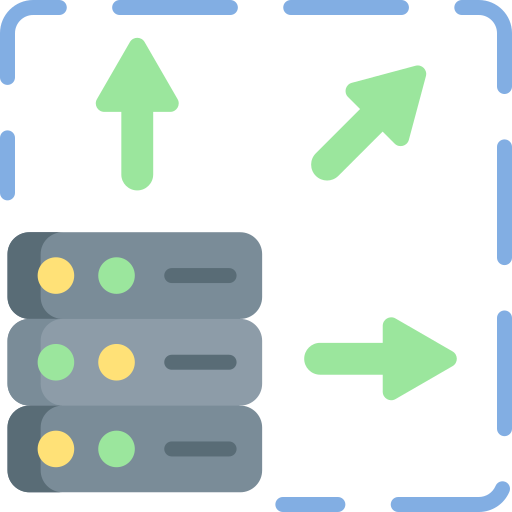
\includegraphics[width=.2\textwidth]{img/icon/scale.png}};

            \node[inner sep=0pt, label=below:Schéma fixe, right=of scale, xshift=1cm] (schema)
                {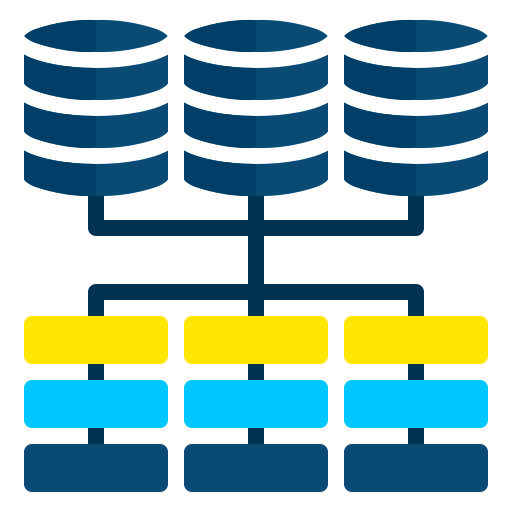
\includegraphics[width=.2\textwidth]{img/icon/database-schema.png}};
        \end{tikzpicture}
        }
    \end{figure}

	\note{
		\begin{itemize}
            \item Difficulté à gérer de grandes quantités de données
            \item Difficulté à gérer des données non structurées ou semi-structurées
            \item Difficulté à évoluer horizontalement (scalabilité)
            \item Complexité des schémas et des relations
    \end{itemize}
	}

\end{frame}

\begin{frame}{En résumé}

	\begin{figure}[htb]
        \centering
        \resizebox{\textwidth}{!}{
        \begin{tikzpicture}

            \node[inner sep=0pt, label=below:Schéma relationnel] (schema) at (0,0)
                {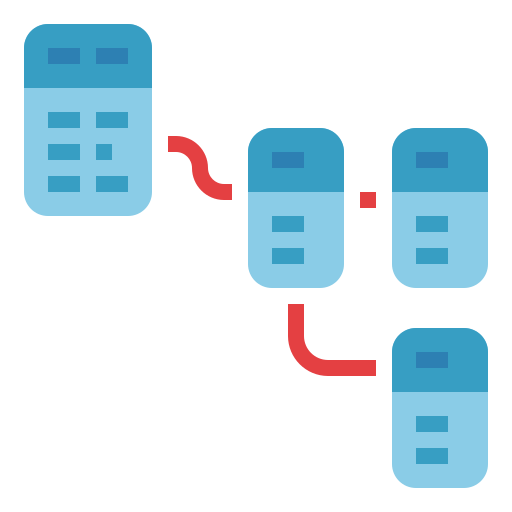
\includegraphics[width=.2\textwidth]{img/icon/relational.png}};

            \node[inner sep=0pt, label=below:Normalisation, right=of schema, xshift=1cm] (normalisation)
                {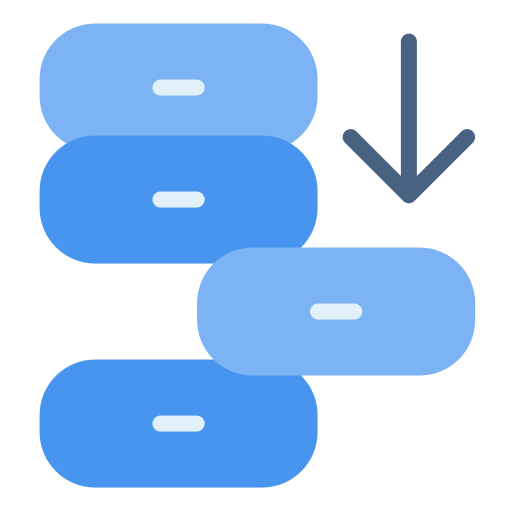
\includegraphics[width=.2\textwidth]{img/icon/normalisation.png}};

            \node[inner sep=0pt, label=below:Langage SQL, right=of normalisation, xshift=1cm] (sql)
                {
\includegraphics[width=.2\textwidth]{img/icon/sql.png}};

            \node[inner sep=0pt, label=below:Vues, right=of sql, xshift=1cm] (view)
                {
\includegraphics[width=.2\textwidth]{img/icon/view.png}};
        \end{tikzpicture}
        }
    \end{figure}

	\note{
		\begin{itemize}
			\item Les bases de données relationnelles organisent les données en \textbf{tables} liées entre elles par des \textbf{clés primaires et étrangères}.
			\item La \textbf{normalisation} est un processus de structuration des données pour \textbf{minimiser la redondance} et \textbf{éviter les anomalies de mise à jour, d'insertion et de suppression}.
			\item Le langage \textbf{SQL} permet de manipuler et de requêter les données dans une base de données relationnelle.
			\item Les \textbf{vues} permettent de \textbf{simplifier les requêtes complexes} et de \textbf{réutiliser des résultats intermédiaires}.
		\end{itemize}
	}

\end{frame}
